\chapter{\label{ch:2-litreview}Biological background} % 808 words

\minitoc

\begin{figure}[h]
	\centering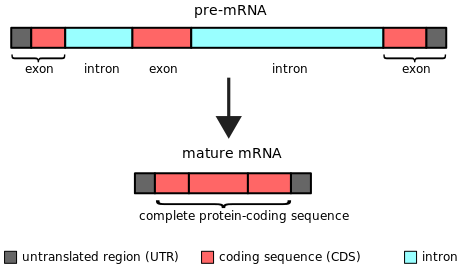
\includegraphics[width=0.9\textwidth]{../visualizations/ch2-biobackground/pre-mrna2mrna.png} 
	\caption
	{The process of splicing \cite{img:mrna}. Introns are removed from the pre-mRNA to obtain the mature mRNA only consisting of exons. Apart from coding regions, exons may also consist of non-coding untranslated regions (UTRs). Like introns, UTRs influence gene expression. 
	}
	\label{fig:pre-mrna2mrna}
\end{figure}

Gene expression is fundamental to all life. It is the process whereby a sequence of nucleotides, a gene, is used to direct the synthesis of a functional gene product (protein, functional RNA). Gene expression occurs in two steps: during transcription, the DNA is transcribed into messenger RNA (mRNA) and during translation, the mRNA is decoded into gene products.\\
In more detail, during transcription an initially transcribed precursor mRNA (pre-RNA) is translated into a mature RNA. 
The majority of sequence information (>90\%) in the pre-RNA is contained in long, non-coding regions, introns, which flank the exons (who are predominantly coding regions). 
%This process, splicing, is motivated by DNA being made up of exons (predominantly coding regions), and, typically longer, introns (non-coding regions).
Only exons are contained in the mature mRNA. Introns are still contained in the initially transcribed precursor mRNA (pre-mRNA). However, they are spliced out by the spliceosome to form the mature mRNA (see Figure \ref{fig:pre-mrna2mrna}). The spliceosome is a complex molecular machine consisting of as many as 150 proteins \cite{splicing_current_perspectives}. The previous location of an intron in the transcript where two exons adjoin each other is called a splice junction or splice site.

\begin{figure}[h]
	\centering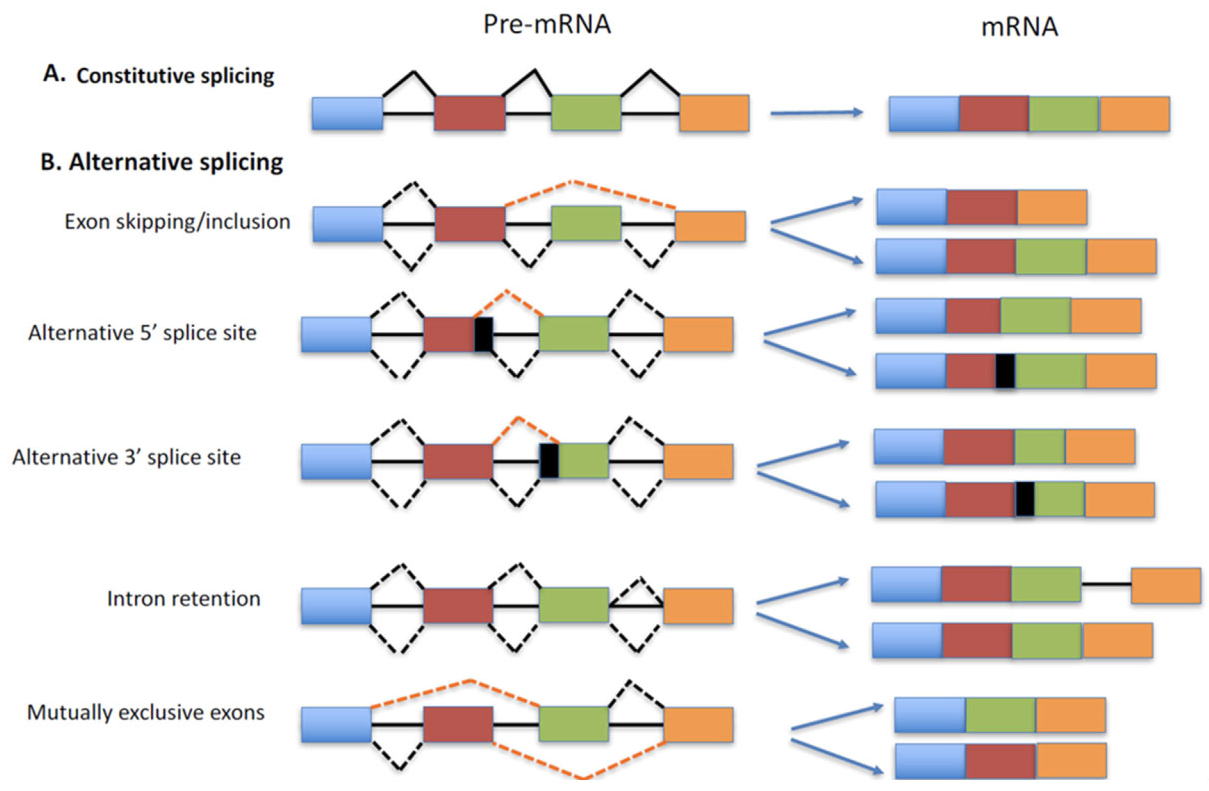
\includegraphics[width=1\textwidth]{../visualizations/ch2-biobackground/alternative_splicing_forms.png} 
	\caption
	{The most common forms of alternative splicing and the resulting different possible mature mRNAs \cite{img:altsplicingforms}.
	}
	\label{fig:altsplicingforms}
\end{figure}

Exons which are always included in the mRNA are called constitutive exons. However, 95\% of human genes with multiple exons are alternatively spliced, that is, they may only sometimes be included, or may be included with different splice sites. Alternative splicing results in the generation of multiple transcripts from a gene. The most common types of alternative splicing in higher eukaryotes are \cite{commonsplicing1}\cite{commonsplicing2}:

\begin{itemize}
\item Cassete exons are exons which are sometimes included in the mature mRNA and sometimes skipped. This is the most common form of alternative splicing in higher eukaryotes (so also humans), accounting for roughly 40\% of all AS splicing events \cite{splicing_current_perspectives}.
\item Exons with an alternative 3' or 5' splice-site. The 3' splice site or splice junction is the end of the exon towards the 3' end of the RNA strand (typically visualized as falling to the right of the sequence). The 5' splice site or splice junction is the end of the exon towards the 5' end of the RNA strand (typically visualized as falling to the left of the sequence). An alternative 3' or 5' splice-site may be located deeper inside the exon or outside the exon in a typically intronic region. Alternative 3' and 5' site splicing respectively constitute approximately 18\% and 8\% of all AS splicing events in higher eukaryotes \cite{splicing_current_perspectives}. 
\item intron retention, that is, when an intron between exons is not spliced out. It accounts for roughly 5\% of AS activity in higher eukaryotes \cite{splicing_current_perspectives}.
\end{itemize}


Different forms of alternative splicing are visualized in Figure \ref{fig:altsplicingforms}. More complex forms of alternative splicing, such as mutually exclusive exons, also exist, but they are currently believed to be less common. Alternative splicing occurs in nearly all organisms that carry out pre-mRNA splicing as such as plants or animals and its frequency varies across organisms \cite{splicing_current_perspectives}. 
\subsubsection{Why does alternative splicing occur?}
Alternative splicing enables a single gene to encode multiple protein variants. This massively contributes to proteomic diversity. For instance, the roughly 20,000 human protein-coding genes are estimated to encoder over 100,000 different proteins \cite{splicing_current_perspectives}.

Alternative splicing may also speed up the rate of evolutionary adaption. Due to alternative splicing, a gene may evolve to fulfil a different functionality without first needing to evolve a separate copy of the same gene. \cite{bretschneiderphdthesis}
\subsubsection{How is alternative splicing regulated?}
Alternative splicing was discovered 40 years ago \cite{discoveryofsplicing}, but the molecular mechanisms governing it are still poorly understood. It is known that the spliceosome recognizes exon-intron boundaries based on the 5' and 3' splice sites, the branch site located in roughly the middle of the exon, and the polypyrimidine tract located upstream of the 3' splice site. However, estimates suggest that these four factors only account for half of the information required to determine splicing behaviour. The rest is likely accounted for by intronic or exonic, cis-acting sequences of the pre-mRNA which bind to trans-acting factors. These cis-acting sequences are usually 4-18 nucleotide long and classified as exonic splicing enhancers or silencers \cite{splicing_current_perspectives}.
However, the dynamic interaction between cis-acting and trans-acting factors is highly complex, new factors are still being found and thus a lot more work needs to be done if we want to fully understand alternative splicing.

%interesting papers for this:
%https://www.ncbi.nlm.nih.gov/pmc/articles/PMC4648177/
%https://onlinelibrary.wiley.com/doi/epdf/10.1002/bies.20692
%https://www.ncbi.nlm.nih.gov/pmc/articles/PMC4360811/#:~:text=Constitutive%20splicing%20is%20the%20process,various%20forms%20of%20mature%20mRNA.
\subsubsection{What happens when splicing is misregulated?}
Since alternative splicing is such a fundamental mechanism, its correct execution is crucial. Defects in splicing are typically caused by genomic sequence variations leading to misregulation of the splicing process. An estimated 9\%-30\% of Mendelian disorders may act through disruption of splicing \cite{comparison} and up to 50\% of known disease-mutations in humans are associated with it \cite{50diseasessplicing}. 
Splice variants have been shown to be biomarkers for multiple types of cancers \cite{cancer} \cite{splicingcausescancer}. As a result, alternative splicing has also been suggested as a biomarker and potential target for drug discovery \cite{drugdiscoverysplicing}. \\

% https://www.sciencedirect.com/science/article/pii/S001457930500253X -- 50% mutation disease from splicing
% big nature splicing in disease paper: https://www.nature.com/articles/nrg2164?cacheBust=1508215213365

% add these caner quoations
% Alternative splicing of fibroblast growth factor receptor 2 (FGF-R2) in human prostate cancer, -1997 meh
%Modification of alternative splicing pathways as a potential approach to chemotherapy,
% Discovery of novel splice forms and functional analysis of cancer-specific alternative splicing in human expressed sequences - done
% Computational analysis and experimental validation of tumor-associated alternative RNA splicing in human cancer - 
% many human genetic diseases: Pre-mRNA splicing and human disease
\subsubsection{Importance of understanding splicing}
Thus, there is great interest in better understanding the mechanisms underpinning alternative splicing. Due to rapid advances in RNA sequencing technologies, it is now possible to sequence the genome of a patient within a day. However, the genomic variants (compared to a reference genome) observed in patients are often variants of unknown significance. \cite{bretschneiderphdthesis} That is, it is unknown whether these variants are pathogenic or benign. An improved understanding of alternative splicing may improve the classification of genomic variants and help with the diagnosis of patients, especially those with rare genomic diseases.
